%
% fig/napoleon.tex -- Napoleon-Dreieck am konkreten Beispiel
% A = 8 + 20i, B = 28 + 22i, C = 17 + 25i (gemaess Praesentation).
% Wir verschieben den Schwerpunkt in den Ursprung und skalieren mit 0.2,
% damit das Bild auf die Seite passt.
%
\begin{figure}
\centering
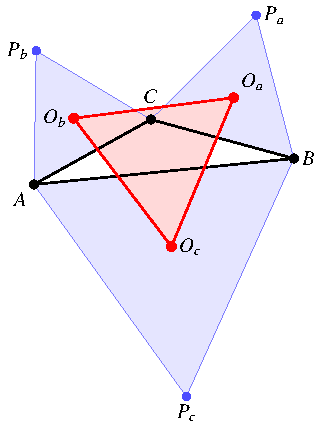
\includegraphics{papers/konstruktion/images/napoleon.pdf}
\caption{Konstruktion zum Satz von Napoleon am Beispiel
$A = 8 + 20i$, $B = 28 + 22i$, $C = 17 + 25i$.
Über jeder Seite des Ausgangsdreiecks $ABC$ (schwarz) wird ein
gleichseitiges Dreieck nach aussen errichtet (blau).
Die Schwerpunkte $O_a$, $O_b$, $O_c$ dieser drei aussen errichteten
Dreiecke bilden das Napoleon-Dreieck (rot), das stets gleichseitig ist.
\label{komplex:figure:napoleon}}
\end{figure}
